\section{Varianzanalyse}

\subsection{Kovarianzanalyse}

\begin{karte}{Varianzanalyse vs. Kovarianzanalyse}
Kovarianzanalyse: Analyse ob die erklärenden Variablen sowohl quantitativ als auch qualitativ (kategoriell) sind.

Varianzanalyse: Analyse ob die erklärenden Variablen ausschließlich qualitative Größen sind.
\end{karte}

\begin{karte}{LRM mit Dummy-Variablen}
Sei \(y_i\) das Ergbebnis, \(x_{i1}\) die erklärende Variable und \(d_i = 0\), falls das Objekt zur ersten 
Gruppe gehört, \(d_i = 1\), falls es zur zweiten Gruppe gehört. 

Mögliche lineare Regressionsmodelle: 
\begin{itemize}
    \item Gleiche Regressionsgerade für beide Gruppen: \(y = \beta_0 \cdot \mathds{1} + \beta_1 X_1 + \varepsilon\)
    \item Spereate Regressionsgeraden mit gleicher Steigung: \(y = \beta_0 \cdot \mathds{1} + \beta_1 X_1 + \beta_2 D + \varepsilon \)
    \item Seperate Regressionsgeraden: \(y = \beta_0 \cdot \mathds{1} + \beta_1 X_1 + \beta_2 D + \beta_3 X_1:D + \varepsilon\), 
    hier sieht die Designmatrix folgendermaßen aus: 
    \[ X = \left( \mathds{1}, X_1, D, \begin{pmatrix}
        x_{11}\cdot d_1 \\ \vdots \\ x_{n1} d_n
    \end{pmatrix} \right). \]
\end{itemize}
\end{karte}

\begin{karte}{Kodierung qualitativer Größen}
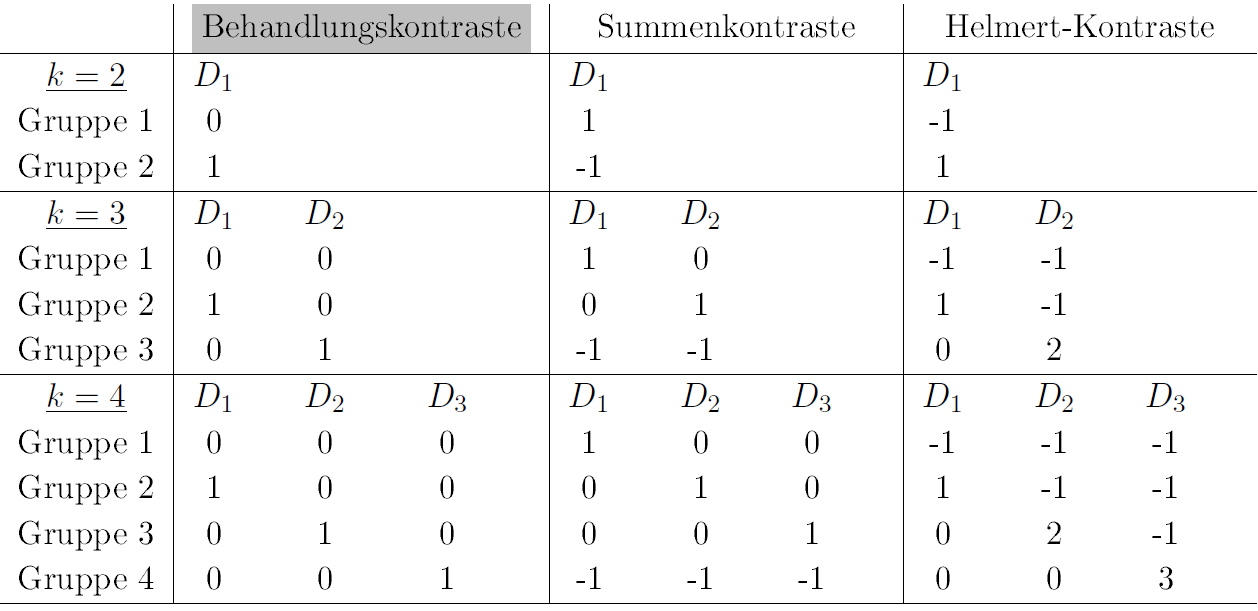
\includegraphics[width=0.9\textwidth]{kodierung-qualitativer-groessen.png}
\end{karte}

\subsection{Einfaktorielle Varianzanalyse}

\begin{karte}{Situation der einfaktoriellen Varianzanalyse}
Seien \(Y_{11}, \ldots, Y_{1n_1}, Y_{21}, \ldots, Y_{2n_2}, Y_{k_1}, \ldots, Y_{k n_k}\) unabhängig, \(Y_{ij} \sim \mathcal{N}(\mu_i, \sigma^2)\).

Getestet wird die Hypothese \(H_0: \mu_1 = \cdots = \mu_k\) gegen \(H_1: \) nicht alle \(\mu_i\) sind gleich.

Wir schreiben \(Y_{ij} = \mu_i + \varepsilon_{ij}\) mit \(\varepsilon_{ij} \sim \mathcal{N}(0, \sigma^2)\).

Dieses Modell lässt sich als LRM schreiben 
\[ \begin{pmatrix}
    Y_{11} \\ \vdots \\ Y_{k n_k}
\end{pmatrix} = \begin{pmatrix}
    \mathds{1} & 0 & & 0 \\
    0 & \mathds{1} & & \vdots \\
    \vdots & 0 & \ddots & 0 \\
    \vdots & \vdots & & \mathds{1}
\end{pmatrix} \begin{pmatrix}
    \mu_1 \\ \vdots \\ \mu_k
\end{pmatrix} + \begin{pmatrix}
    \varepsilon_{11} \\ \vdots \\ \varepsilon_{k n_k}
\end{pmatrix}. \]
\end{karte}

\begin{karte}{Kleinste-Quadrate-Schätzer Varianzanalyse}
\[y_{i+} := \sum_{j=1}^{n_i} y_{ij}, \quad \bar{y}_{i+} := \frac{1}{n_i} y_{i+}. \]
Dann gilt 
\[ X^T X = \begin{pmatrix}
    n_1 & & 0 \\
    & \ddots & \\
    0 & & n_k
\end{pmatrix}, X^T Y = \begin{pmatrix}
    Y_{1+} \\ \vdots \\ Y_{k+}
\end{pmatrix} \Rightarrow \hat{\beta} = (X^T X)^{-1} X^T Y = \begin{pmatrix}
    \bar{Y}_{1+} \\ \vdots \\ \bar{Y}_{k+}
\end{pmatrix}. \]
Es folgt wegen \(\hat{Y} = X \hat{\beta}\)
\[ \hat{Y} = (\hat{Y}_{1+}, \ldots, \hat{Y}_{1+}, \ldots, \hat{Y}_{k+}, \ldots, \hat{Y}_{k+})^T, \hat{\varepsilon}_{ij} = Y_{ij} - \bar{Y}_{i+}, \]
\[ \hat{\varepsilon}^T \hat{\varepsilon} = \sum_{i=1}^k \sum_{j=1}^{n_i} (Y_{ij} - \bar{Y}_{i+})^2, \hat{\sigma}_{ML}^2 = \frac{\hat{\varepsilon}^T \hat{\varepsilon}}{n}, \hat{\sigma}^2 = \frac{\hat{\varepsilon}^T \hat{\varepsilon}}{n-k}. \]
\end{karte}

\begin{karte}{Übliche Kodierungen der einfaktoriellen ANOVA}
Das lineare Modell wird so in der Praxis nicht verwendet. Das liegt daran, dass in der Designmatrix kein Intercept vorkommt. 
Stattdessen verwenden wir dies: 
\[ Y_{ij} = \mu + \alpha_i + \varepsilon_{ij}. \]
\end{karte}

\begin{karte}{Modell 1: \(\alpha_1 = 0\)}
Modell 1: Setze \(\alpha_1 = 0\). Gruppe 1 ist dann Kontrollgruppe mit Erwartungswert \(1\), die anderen haben Erwartungswert \(\mu + \alpha_i\).
\(\beta = (\mu, \alpha_2, \ldots, \alpha_k)^T\).
\end{karte}

\begin{karte}{Modell 2: Summenrestriktion}
Modell 2: Summenrestriktion. 
Hier nehmen wir zusätzlich an, dass \(n_1 = \cdots = n_k\) gilt. 
In diesem Fall lautet die Summenrestriktion \(\sum n_i \alpha_i = \sum \alpha_i = 0\).
\[ X := \begin{pmatrix}
    1 & \mathds{1} & 0 & & 0\\
    \vdots & 0 & \mathds{1} & & \vdots \\
    \vdots & \vdots & 0 & \ddots & \vdots \\
    \vdots & \vdots & 0 & & \mathds{1} \\
    1 & -\mathds{1} & -\mathds{1} & \cdots & -\mathds{1}
\end{pmatrix} \]
Für den Erwartungswert der \(i\)-ten Gruppe erhält man 
\((X \beta)_{(i-1)\cdot n_1 + j} = \mu + \alpha_i\). Für den Erwartungswert der \(k\)-ten Gruppe hingegen 
\((X \beta)_{(k-1)\cdot n_1 + j} = \mu - \alpha_1 - \cdots - \alpha_{k-1}\).
Also muss \(\alpha_k = -\sum_{i=1}^{k-1} \alpha_i\) gelten. Somit gilt \(\sum \alpha_i = 0\).
\end{karte}

\begin{karte}{Parameterschätzung in Modell 1}
Es gilt 
\[ X^T X = \begin{pmatrix}
    n & n_2 & n_3 & \cdots & n_k \\
    n_2 & n_2 & 0 & \cdots & 0 \\
    n_3 & 0 & n_3 & \ddots & \vdots \\
    \vdots & \vdots & \ddots & \ddots & 0 \\
    n_k & 0 & \cdots & 0 & n_k
\end{pmatrix}, (X^T X)^{-1} = \frac{1}{n_1} \begin{pmatrix}
    1 & -1 & \cdots & \cdots & -1 \\
    -1 & \frac{n_1 + n_2}{n_2} & 1 & \cdots & 1 \\
    \vdots & 1 & \frac{n_1 + n_3}{n_3} & \ddots & \vdots \\
    \vdots & \vdots & \ddots & \ddots & 1 \\
    -1 & 1 & \cdots & 1 & \frac{n_1 + n_k}{n_k}
\end{pmatrix}. \]
Weiter gilt 
\[ X^T Y = \begin{pmatrix}
    \sum_{i,j} Y_{i,j} \\
    \sum_j Y_{2,j} \\
    \vdots \\
    \sum_j Y_{k,j}
\end{pmatrix} =: \begin{pmatrix}
    Y_{++} \\
    Y_{2+} \\
    \vdots \\
    Y_{k+}
\end{pmatrix} \Rightarrow \hat{\beta} = 
\begin{pmatrix}
    \hat{\mu} \\
    \hat{\alpha}_2 \\
    \vdots \\
    \hat{\alpha}_k
\end{pmatrix} = (X^T X)^{-1} X^T Y = \begin{pmatrix}
    \bar{Y}_{1+} \\
    \bar{Y}_{2+} - \bar{Y}_{1+} \\
    \vdots \\
    \bar{Y}_{k+} - \bar{Y}_{1+}
\end{pmatrix}. \]
\end{karte}

\begin{karte}{Parameterschätzung in Modell 2}
Wir erhalten \[ X^T X = n_1 \begin{pmatrix}
    k & 0 & \cdots & \cdots & 0 \\
    0 & 2 & 1 & \cdots & 1 \\
    \vdots & 1 & 2 & \ddots & \vdots \\
    \vdots & \vdots & \ddots & \ddots & 1 \\
    0 & 1 & \cdots & 1 & 2
\end{pmatrix}, (X^T X)^{-1} = \frac{1}{k n_1} \begin{pmatrix}
    1 & 0 & \cdots & \cdots & 0 \\
    0 & k-1 & -1 & \cdots & -1 \\
    \vdots & -1 & k-1 & \ddots & \vdots \\
    \vdots & \vdots & \ddots & \ddots & -1 \\
    0 & -1 & \cdots & -1 & k-1
\end{pmatrix}. \]
Somit gilt 
\[ X^T Y = \begin{pmatrix}
    Y_{++} \\ Y_{1+} - Y_{k+} \\ \vdots \\ Y_{k-1,+} - Y_{k+} 
\end{pmatrix} \Rightarrow \hat{\beta} = \begin{pmatrix}
    \hat{\mu} \\ \hat{\alpha}_1 \\ \vdots \\ \hat{\alpha}_{k-1}
\end{pmatrix} = \begin{pmatrix}
    \bar{Y}_{++} \\
    \bar{Y}_{1+} - \bar{Y}_{++} \\
    \vdots \\
    \bar{Y}_{k-1,+} - \bar{Y}_{++}
\end{pmatrix}. \]

Setzt man \(\hat{\alpha}_k := \bar{Y}_{k+} - \bar{Y}_{++}\), so folgt 
\[ \sum_{i=1}^k \hat{\alpha}_i = \sum_{i=1}^k \bar{Y}_{i+} - k\cdot \bar{Y}_{++} = \frac{1}{n_1} \sum_{i=1}^k Y_{i+} - \frac{1}{n_1} \cdot Y_{++} = 0. \]
Die Schätzer erfüllen also ebenfalls die Summenrestriktion.
\end{karte}

\begin{karte}{Der globale \(F\)-Test 1}
Getestet wird die Hypothese \(H_0: \mu_1 = \cdots = \mu_k\) bzw. \(H_0: \alpha_1 = \cdots = \alpha_k = 0\) in Modell 1 bzw. 2.
Bei den Modellen 1 und 2 vergleicht man z. B. das Obermodell \(Y_{ij} = \mu + \alpha_i + \varepsilon_{ij}\) 
mit dem Teilmodell \(Y_{ij} = \mu + \varepsilon_{ij}\).

Als Testgröße wählen wir 
\[ F = \frac{(\mathrm{RSS}_1 - \mathrm{RSS})/(k-1)}{\mathrm{RSS}/(n-k)} \sim F_{k-1,n-k} \text{ unter } H_0. \]
Es gilt \(\mathrm{RSS}_1 = \mathrm{TSS} = \sum_{i,j} (Y_{ij} - \bar{Y}_{++})^2\).
Für das Obermodell gilt 
\[ \hat{Y}_{ij} = \bar{Y}_{i+} \]
und somit 
\[ \mathrm{RSS} = \sum_{i=1}^k \sum_{j=1}^{n_i} (Y_{ij} - \bar{Y}_{i+})^2 =: \mathrm{SQI}. \]
SQI steht für \gqq{Summe der Quadrate innerhalb (der Gruppen)}. 
Es gilt \(\mathrm{TSS} = \mathrm{SQI} + \mathrm{SQZ}\) mit \(\mathrm{SQZ} = \sum_{i=1}^k n_i (\bar{Y}_{i+} - \bar{Y}_{++})^2\). 

Somit gilt \[\mathrm{RSS}_1 - \mathrm{RSS} = \mathrm{TSS} - \mathrm{SQI} = \mathrm{SQZ}. \]
\end{karte}

\begin{karte}{Der globale \(F\)-Test 2}
Also lässt sich \(F\) schreiben als \[F = \frac{\mathrm{SQZ}/(k-1)}{\mathrm{SQI}/(n-k)}. \]
Der Testentscheid lautet 
\begin{align*}
    H_0 \text{ verwerfen, falls } & F \geq F_{k-1,n-k;1-\alpha}, \\
    H_0 \text{ nicht verwerfen, falls } & F < F_{k-1,n-k;1-\alpha}.
\end{align*}
\end{karte}

\subsection{Multiple Vergleiche}

\begin{karte}{Multiple Tests mit Bonferroni-Korrektur}
Es seien \(m\) Hypothesen zu testen. Sei 
\begin{align*}
    S &:= \set{\text{mindestens einer der \(m\) Tests ist signifikant}}, \\
    S_l &:= \set{\text{der \(l\)-te Test ist signifikant}} \quad (l=1,\ldots, m).
\end{align*}
Für jeden Test mit der Nullhypothese \(H_{0,l}\) gilt: \(P_{H_{0,l}}(S_l) = \alpha\).
Die globale Nullhypothese \(H_0\) besagt, dass alle \(m\) Nullhypothesen \(H_{0,l}\) gelten.
\end{karte}

\begin{karte}{Tukey-Methode (Simultane Konfidenzintervalle)}
Sei \(W_1, \ldots, W_k \oversett{uiv}{\sim} \mathcal{N}(\mu, \sigma^2)\) und \(R := \max_i W_i - \min_i W_i\),
Weiter sei \(V\sim \chi_k^2\) und \(V, W_1, \ldots, W_k\) unabhängig. Für \(S^2 := \sigma^2 V/\nu\) 
gilt dann \(E(S^2) = \sigma^2\) und \(Q_{k,\nu} := R/S\) heißt \textit{studentisierte Spannweite}.

Sei \(n_1 = \ldots = n_k\) und \(\mu_i\) seien die wahren Erwartungswerte in den \(k\) Gruppen. Dann gilt 
\[ P(\bar{Y}_{i+} - \bar{Y}_{j+} - D \leq \mu_i - \mu_j \leq \bar{Y}_{i+} - \bar{Y}_{j+} + D) = 1-\alpha, \]
wobei 
\[ D = Q_{k,n-k;1-\alpha} \cdot \sqrt{\frac{\mathrm{SQI}}{n_1(n-k)}}. \]
Hier bezeichnet \(Q_{k,\nu;p}\) das \(p\)-Quantil der Verteilung der studentisierten Spannweite \(Q_{k,\nu}\).

Hypothese: \(H_0^{i,j}: \mu_i = \mu_j\)
Testentscheid: Verwerfe \(H_0^{i,j}\), falls \(0 \not\in I^{i,j}\).

Das so definierte multiple Testverfahren hat ein multiples Signifikanzniveau \(\leq \alpha\): \(FWE_s \leq \alpha\).
\end{karte}

\subsection{Zweifaktorielle ANOVA}

\begin{karte}{Zweifaktorielle ANOVA Modell}
\[ Y_{ijk} = \mu + \alpha_i + \beta_j + \gamma_{ij} + \varepsilon_{ijk}, i=1,\ldots, I, j=1,\ldots, J, k = 1, \ldots, n_{ij}, \varepsilon_{ijk} \sim \mathcal{N}(0, \sigma^2). \]

Summenrestriktion: 
\[ \sum \alpha_i = 0, \sum \beta_j = 0, \sum_{i=1}^I \gamma_{ij} = 0, \sum_{j=1}^J \gamma_{ij} = 0. \]
Somit liegen tatsächlich (eine redundant) \(I + J + 1\) Restriktionen vor. 
\end{karte}

\begin{karte}{\(F\)-Test der zweifaktoriellen Varianzanalyse}
Teilmodell ohne Interaktion: 
\(y_{ijk}=\mu + \alpha_i + \beta_j + \varepsilon_{ijk}\)
Anzahl der Parameter: Teilmodell \(r = (I-1) + (J-1) + 1\), Obermodell \(p=I \cdot J\).

Führt man einen \(F\)-Test des Teilmodells gegen das Obermodell durch, so besitzt bei Gültigkeit des 
Teilmodells eine \(F\)-Verteilung mit \(p-r = IJ - I -J + 1\) Zählerfreiheitsgeraden und \(n-p = n - IJ\) 
Nennerfreiheitsgeraden. 
\end{karte}

\begin{karte}{Streuungszerlegung im zweifaktoriellen ANOVA-Modell}
Im zweifaktoriellen ANOVA-Modell mit \(n_{ij}=K\) gilt die Streuungszerlegung 
\[ \mathrm{SS}_{\mathrm{TOTAL}} = \mathrm{SS}_A + \mathrm{SS}_B + \mathrm{SS}_{AB} + \mathrm{SS}_E, \]
wobei 
\begin{align*}
    \mathrm{SS}_{\mathrm{TOTAL}} &:= \sum_{i=1}^I \sum_{j=1}^J \sum_{k=1}^K (Y_{ijk} - \underbrace{\hat{Y}_{+++}}_{=\hat{\mu}})^2,\\
    \mathrm{SS}_A &:= JK \sum_{i=1}^I (\bar{Y}_{++} - \bar{Y}_{+++})^2, \quad \mathrm{SS}_B := IK \sum_{j=1}^J (\bar{Y}_{+j+} - \bar{Y}_{+++})^2, \\
    \mathrm{SS}_{AB} &:= K \sum_{i=1}^I \sum_{j=1}^J (\bar{Y}_{ij+} - \bar{Y}_{i++} - \bar{Y}_{+j+} + \bar{Y}_{+++})^2, \\
    \mathrm{SS}_E &:= \sum_{i=1}^I \sum_{j=1}^J \sum_{k=1}^K (Y_{ijk} - \bar{Y}_{ij+})^2.
\end{align*}
\end{karte}

\begin{karte}{Zweifaktorielle ANOVA Quadratsummen unter \(H_A, H_B, H_{AB}\)}
Bei der zweifaktoriellen ANOVA mit \( n_{ij} = K \) gilt: 
\begin{enumerate}
    \item \(\frac{\mathrm{SS}_E}{\sigma^2} \sim \chi_{IJ (K-1)}^2\).
    \item Unter \(H_A: \alpha_i = 0\) für \( i = 1, \ldots, I\) gilt \( \frac{\mathrm{SS}_A}{\sigma^2} \sim \chi_{I-1}^2\).
    \item Unter \(H_B: \beta_j = 0\) für \(j=1, \ldots, J\) gilt \(\frac{\mathrm{SS}_B}{\sigma^2} \sim \chi_{J-1}^2\).
    \item Unter \(H_{AB} : \gamma_{ij} = 0\) gilt \(\frac{\mathrm{SS}_{AB}}{\sigma^2} \sim \chi_{(I-1)(J-1)}^2\).
    \item Alle Quadratsummen sind unabhängig.
\end{enumerate}
\end{karte}